\subsection{Combining Parameter}

Thus far, we have not seen type B regions, that are not caused by overlapping type A regions.
We now want to change multiple parameters at the same time to imitate the function of the original model better.
For this, we introduce new parameters, $p_x$ and $p_y$, and define the actual model parameters dependent on those two.

\subsubsection{Defining $a_R = 1 + p_x$, $b_R = 2 \cdot px$, and $c_L = p_y$}

\todo{better imitation but nothing was found}

\subsubsection{Defining $a_R = 1 + 2 \cdot p_x$, $b_R = px$, and $c_L = p_y$}

This definition of $a_R$ and $b_R$ is similar to before, but now $p_x$ has double the effect on $a_R$ and half the effect on $b_R$.
It was created by accident since it does not imitate the original model as nicely as before.
\Cref{fig:quadratic.full.2aR1bR_cL.2d.full} shows the 2D scan of the different periods.
Regions we will have a closer look at, are marked with red rectangles.

\begin{figure}
    \centering
    \includegraphics[width=0.6\textwidth]{21_010_Quadratic_2aR1bR_cL/2D_Period_Selected/result.png}
    \caption{2D Scan of Periods of Quadratic Model with ...}
    \label{fig:quadratic.full.2aR1bR_cL.2d.full}
\end{figure}

The first enhanced region, shown in \Cref{fig:quadratic.full.2aR1bR_cL.2d.1}, has two areas with stable cycles of period 6 that overlap.
\Cref{fig:quadratic.regions.2aR1bR_cL.2d.1} shows the borders of the two regions.
It was created by halving the model and scanning for the borders of regions of different periods.
We will see that the bottom area is a type B area, and therefore the period in the halved model is double the period in the full model.

\begin{figure}
    \centering
    \begin{subfigure}{0.4\textwidth}
        \centering
        \includegraphics[width=\textwidth]{21_010_Quadratic_2aR1bR_cL/P6/2D_Period_P6/result.png}
        \caption{Periods}
        \label{fig:quadratic.full.2aR1bR_cL.2d.1}
    \end{subfigure}
    \begin{subfigure}{0.4\textwidth}
        \centering
        \includegraphics[width=\textwidth]{21_010_Quadratic_2aR1bR_cL/P6/2D_Regions_P6/result.png}
        \caption{Period Regions}
        \label{fig:quadratic.regions.2aR1bR_cL.2d.1}
    \end{subfigure}
    \caption{2D Scans of First Marked Region}
\end{figure}

\Cref{fig:quad.full.2aR1bR_cL.1.Cobwebs} shows cobweb diagrams at the three points marked in \Cref{fig:quadratic.full.2aR1bR_cL.2d.1,fig:quadratic.regions.2aR1bR_cL.2d.1}.
At point $A$, we have two stable coexisting cycles of period 6 with symbolic sequences $\A\B\C^3D$ and $\A^3\B\C\D$.
You can see them in \Cref{fig:quad.full.2aR1bR_cL.1.CobwebA}.
This region is therefore a type B region since we have two coexisting cycles that are symmetric by rotation.
At point $C$, we only have one stable cycle of period 6 with symbolic sequence $\A^2\B\C^3\D$.
\Cref{fig:quad.full.2aR1bR_cL.1.CobwebC} shows this cycle.
The upper region, therefore, is a type A region.
Both these regions overlap like in the original model.
\Cref{fig:quad.full.2aR1bR_cL.1.CobwebB} shows the stable cycles at point $C$ in the overlapping area.
\todo{similarity to overlap in og model}

\begin{figure}
    \centering
    \begin{subfigure}{0.3\textwidth}
        \centering
        \includegraphics[width=\textwidth]{21_010_Quadratic_2aR1bR_cL/P6/Cobweb_P6_A/result.png}
        \caption{At Point A}
        \label{fig:quad.full.2aR1bR_cL.1.CobwebA}
    \end{subfigure}
    \begin{subfigure}{0.3\textwidth}
        \centering
        \includegraphics[width=\textwidth]{21_010_Quadratic_2aR1bR_cL/P6/Cobweb_P6_B/result.png}
        \caption{At Point B}
        \label{fig:quad.full.2aR1bR_cL.1.CobwebB}
    \end{subfigure}
    \begin{subfigure}{0.3\textwidth}
        \centering
        \includegraphics[width=\textwidth]{21_010_Quadratic_2aR1bR_cL/P6/Cobweb_P6_C/result.png}
        \caption{At Point C}
        \label{fig:quad.full.2aR1bR_cL.1.CobwebC}
    \end{subfigure}
    \caption{Cobwebs at Different Points}
    \label{fig:quad.full.2aR1bR_cL.1.Cobwebs}
\end{figure}

The second, lower, enhanced region has two areas with stable cycles of period 8 that overlap.
\Cref{fig:quadratic.full.2aR1bR_cL.2d.2} shows that region, while \Cref{fig:quadratic.regions.2aR1bR_cL.2d.2} shows the borders of the two areas, like before.

\begin{figure}
    \centering
    \begin{subfigure}{0.4\textwidth}
        \centering
        \includegraphics[width=\textwidth]{21_010_Quadratic_2aR1bR_cL/P8/2D_Period_P8/result.png}
        \caption{Periods}
        \label{fig:quadratic.full.2aR1bR_cL.2d.2}
    \end{subfigure}
    \begin{subfigure}{0.4\textwidth}
        \centering
        \includegraphics[width=\textwidth]{21_010_Quadratic_2aR1bR_cL/P8/2D_Regions_P8/result.png}
        \caption{Period Regions}
        \label{fig:quadratic.regions.2aR1bR_cL.2d.2}
    \end{subfigure}
    \caption{2D Scans of Second Marked Region}
\end{figure}

\Cref{fig:quad.full.2aR1bR_cL.2.Cobwebs} shows cobweb diagrams at the three points marked in \Cref{fig:quadratic.full.2aR1bR_cL.2d.2,fig:quadratic.regions.2aR1bR_cL.2d.2}.
We can see that the lower area is again of type B, we have two coexisting stable cycles of period 8 with symbolic sequences $\A^2\B\C^4\D$ and $\A^4\B\C^2\D$.
\Cref{fig:quad.full.2aR1bR_cL.2.CobwebA} shows these cycles at the point $A$.
As before, the other area is of type B and has one stable cycle of period 8 with the symbolic sequence $\A^3\B\C^3\D$.
You can see it in \Cref{fig:quad.full.2aR1bR_cL.2.CobwebC}, it was generated at the point $C$.

\begin{figure}
    \centering
    \begin{subfigure}{0.3\textwidth}
        \centering
        \includegraphics[width=\textwidth]{21_010_Quadratic_2aR1bR_cL/P8/Cobweb_P8_A/result.png}
        \caption{At Point A}
        \label{fig:quad.full.2aR1bR_cL.2.CobwebA}
    \end{subfigure}
    \begin{subfigure}{0.3\textwidth}
        \centering
        \includegraphics[width=\textwidth]{21_010_Quadratic_2aR1bR_cL/P8/Cobweb_P8_B/result.png}
        \caption{At Point B}
        \label{fig:quad.full.2aR1bR_cL.2.CobwebB}
    \end{subfigure}
    \begin{subfigure}{0.3\textwidth}
        \centering
        \includegraphics[width=\textwidth]{21_010_Quadratic_2aR1bR_cL/P8/Cobweb_P8_C/result.png}
        \caption{At Point C}
        \label{fig:quad.full.2aR1bR_cL.2.CobwebC}
    \end{subfigure}
    \caption{Cobwebs at Different Points}
    \label{fig:quad.full.2aR1bR_cL.2.Cobwebs}
\end{figure}

\subsubsection{Mirrored Configuration}

One idea to obtain chains from the overlapping area found above, is to move from the parameter values that are inside this area to parameter values that produce the same function rotated by one branch.
This is equivalent to the function, where parameters $a_L$ and $b_L$ are swapped with $a_R$ and $b_R$ and the parameters $c_L$ and $c_R$ are swapped with an offset of $1.5$.
Let point $A$ be the point inside the overlapping area (point $B$) in \Cref{fig:quadratic.full.2aR1bR_cL.2d.1} and point $A'$ the mirrored configuration, just described.
\Cref{fig:quad.full.2aR1bR_cL_mirr.1.Cobwebsprime}

\begin{figure}
    \centering
    \begin{subfigure}{0.4\textwidth}
        \centering
        \includegraphics[width=\textwidth]{21_012_Quadratic_2aR1bR_mirror/Cobweb_A/result.png}
        \caption{At Point $A$}
        \label{fig:quad.full.2aR1bR_cL_mirr.1.CobwebA}
    \end{subfigure}
    \begin{subfigure}{0.4\textwidth}
        \centering
        \includegraphics[width=\textwidth]{21_012_Quadratic_2aR1bR_mirror/Cobweb_Aprime/result.png}
        \caption{At Point $A'$}
        \label{fig:quad.full.2aR1bR_cL_mirr.1.CobwebAprime}
    \end{subfigure}
    \caption{Cobwebs at Different Points}
    \label{fig:quad.full.2aR1bR_cL_mirr.1.Cobwebsprime}
\end{figure}

Now we choose the parameters $p_x$ and $p_y$ in such a way, that $p_x = p_y = 0$ corresponds to the configuration in point $A$ AND $p_x = p_y = 1$ to the configuration in point $A'$.
While $p_x$ influences $a_L, a_R, b_L,$ and $b_R$, while $p_y$ only influences $c_L$ and $c_R$.
The resulting scan of the periods is \Cref{fig:quadratic.full.2aR1bR_mirr.1.2d.whole}.

\begin{figure}
    \centering
    \includegraphics[width=0.6\textwidth]{21_012_Quadratic_2aR1bR_mirror/2D_Period_Whole/result.png}
    \caption{2D Scan of Periods of Quadratic Model with ...}
    \label{fig:quadratic.full.2aR1bR_mirr.1.2d.whole}
\end{figure}

The behavior of the model at the point $B$ here is equivalent to point $C$ in \Cref{fig:quadratic.full.2aR1bR_cL.2d.1}, therefore its cobweb is omitted here.
The cobwebs of points $C$ and $D$ in \Cref{fig:quad.full.2aR1bR_cL_mirr.1.CobwebsCD} show that there is also the same situation of a type A and a type B area.
At the point $C$ we have one stable cycle of period 6 with the symbolic sequence $\A\B^2\C\D^2$.
At the point $D$ we have two stable cycles of period 6 with the same symbolic sequence $\A\B^2\C\D^2$.
But in that case, they do not overlap, as you can see in \Cref{fig:quadratic.full.2aR1bR_mirr.1.2d.CD}.
Also, the coexisting cycles are situated differently from the original model, where it is characteristic that one cycle runs near the right of a border between two branches, while the other cycle runs near the left of it.

\begin{figure}
    \centering
    \includegraphics[width=0.6\textwidth]{21_012_Quadratic_2aR1bR_mirror/2D_Period_CD/result.png}
    \caption{2D Scan of Periods of Quadratic Model with ...}
    \label{fig:quadratic.full.2aR1bR_mirr.1.2d.CD}
\end{figure}

\begin{figure}
    \centering
    \begin{subfigure}{0.4\textwidth}
        \centering
        \includegraphics[width=\textwidth]{21_012_Quadratic_2aR1bR_mirror/Cobweb_C/result.png}
        \caption{At Point $C$}
        \label{fig:quad.full.2aR1bR_cL_mirr.1.CobwebC}
    \end{subfigure}
    \begin{subfigure}{0.4\textwidth}
        \centering
        \includegraphics[width=\textwidth]{21_012_Quadratic_2aR1bR_mirror/Cobweb_D/result.png}
        \caption{At Point $D$}
        \label{fig:quad.full.2aR1bR_cL_mirr.1.CobwebD}
    \end{subfigure}
    \caption{Cobwebs at Different Points}
    \label{fig:quad.full.2aR1bR_cL_mirr.1.CobwebsCD}
\end{figure}

At the point $E$ we also have a type B area with two coexisting cycles of period 6.
The symbolic sequences of these cycles are $\A^2\B^2\C\D$ and $\A\B\C^2\D^2$ and the cycles are situated like in the original model again.
But this area is not something we are searching for.
The type B areas we are searching for should have the same number of points on their left half as they have on their right half.
Because in the original model, the two type A areas on either side of a type B area behave like in one half of one cycle in the type B area on both halves.
And it has the same period, therefore the points in the type B area must be distributed equally on both halves,
\todo{better explanation - maybe earlier in the original model, reference here}

\begin{figure}
    \centering
    \includegraphics[width=0.6\textwidth]{21_012_Quadratic_2aR1bR_mirror/Cobweb_E/result.png}
    \caption{Cobweb at Point $E$}
    \label{fig:quadratic.full.2aR1bR_mirr.1.CobwebE}
\end{figure}

Repeating the same spiel for the second, lower parameter region for period 8 cycles, we arrive at the scans shown in \Cref{fig:quad.full.2aR1bR_cL_mirr.2.Period}.
The first scan shows the normal model with points in parameter regions of period 8.
We can see from this scan, that these regions are disjunct and therefore don't overlap.
To make sure, there are no type A and type B regions overlapping inside one of the large parameter 8 regions, we half the model and scan again.
This scan is shown in \Cref{fig:quad.full.2aR1bR_cL_mirr.2.Halved}.
As we can see, the regions are either a little lighter or a little darker, but monotone.
This means, that there are no overlapping type A and type B parameter regions.
Therefore we do not investigate this model any further.

\begin{figure}
    \centering
    \begin{subfigure}{0.4\textwidth}
        \centering
        \includegraphics[width=\textwidth]{21_013_Quadratic_2aR1bR_mirror2/2D_Period_Whole/result.png}
        \caption{Full Model}
        \label{fig:quad.full.2aR1bR_cL_mirr.2.whole}
    \end{subfigure}
    \begin{subfigure}{0.4\textwidth}
        \centering
        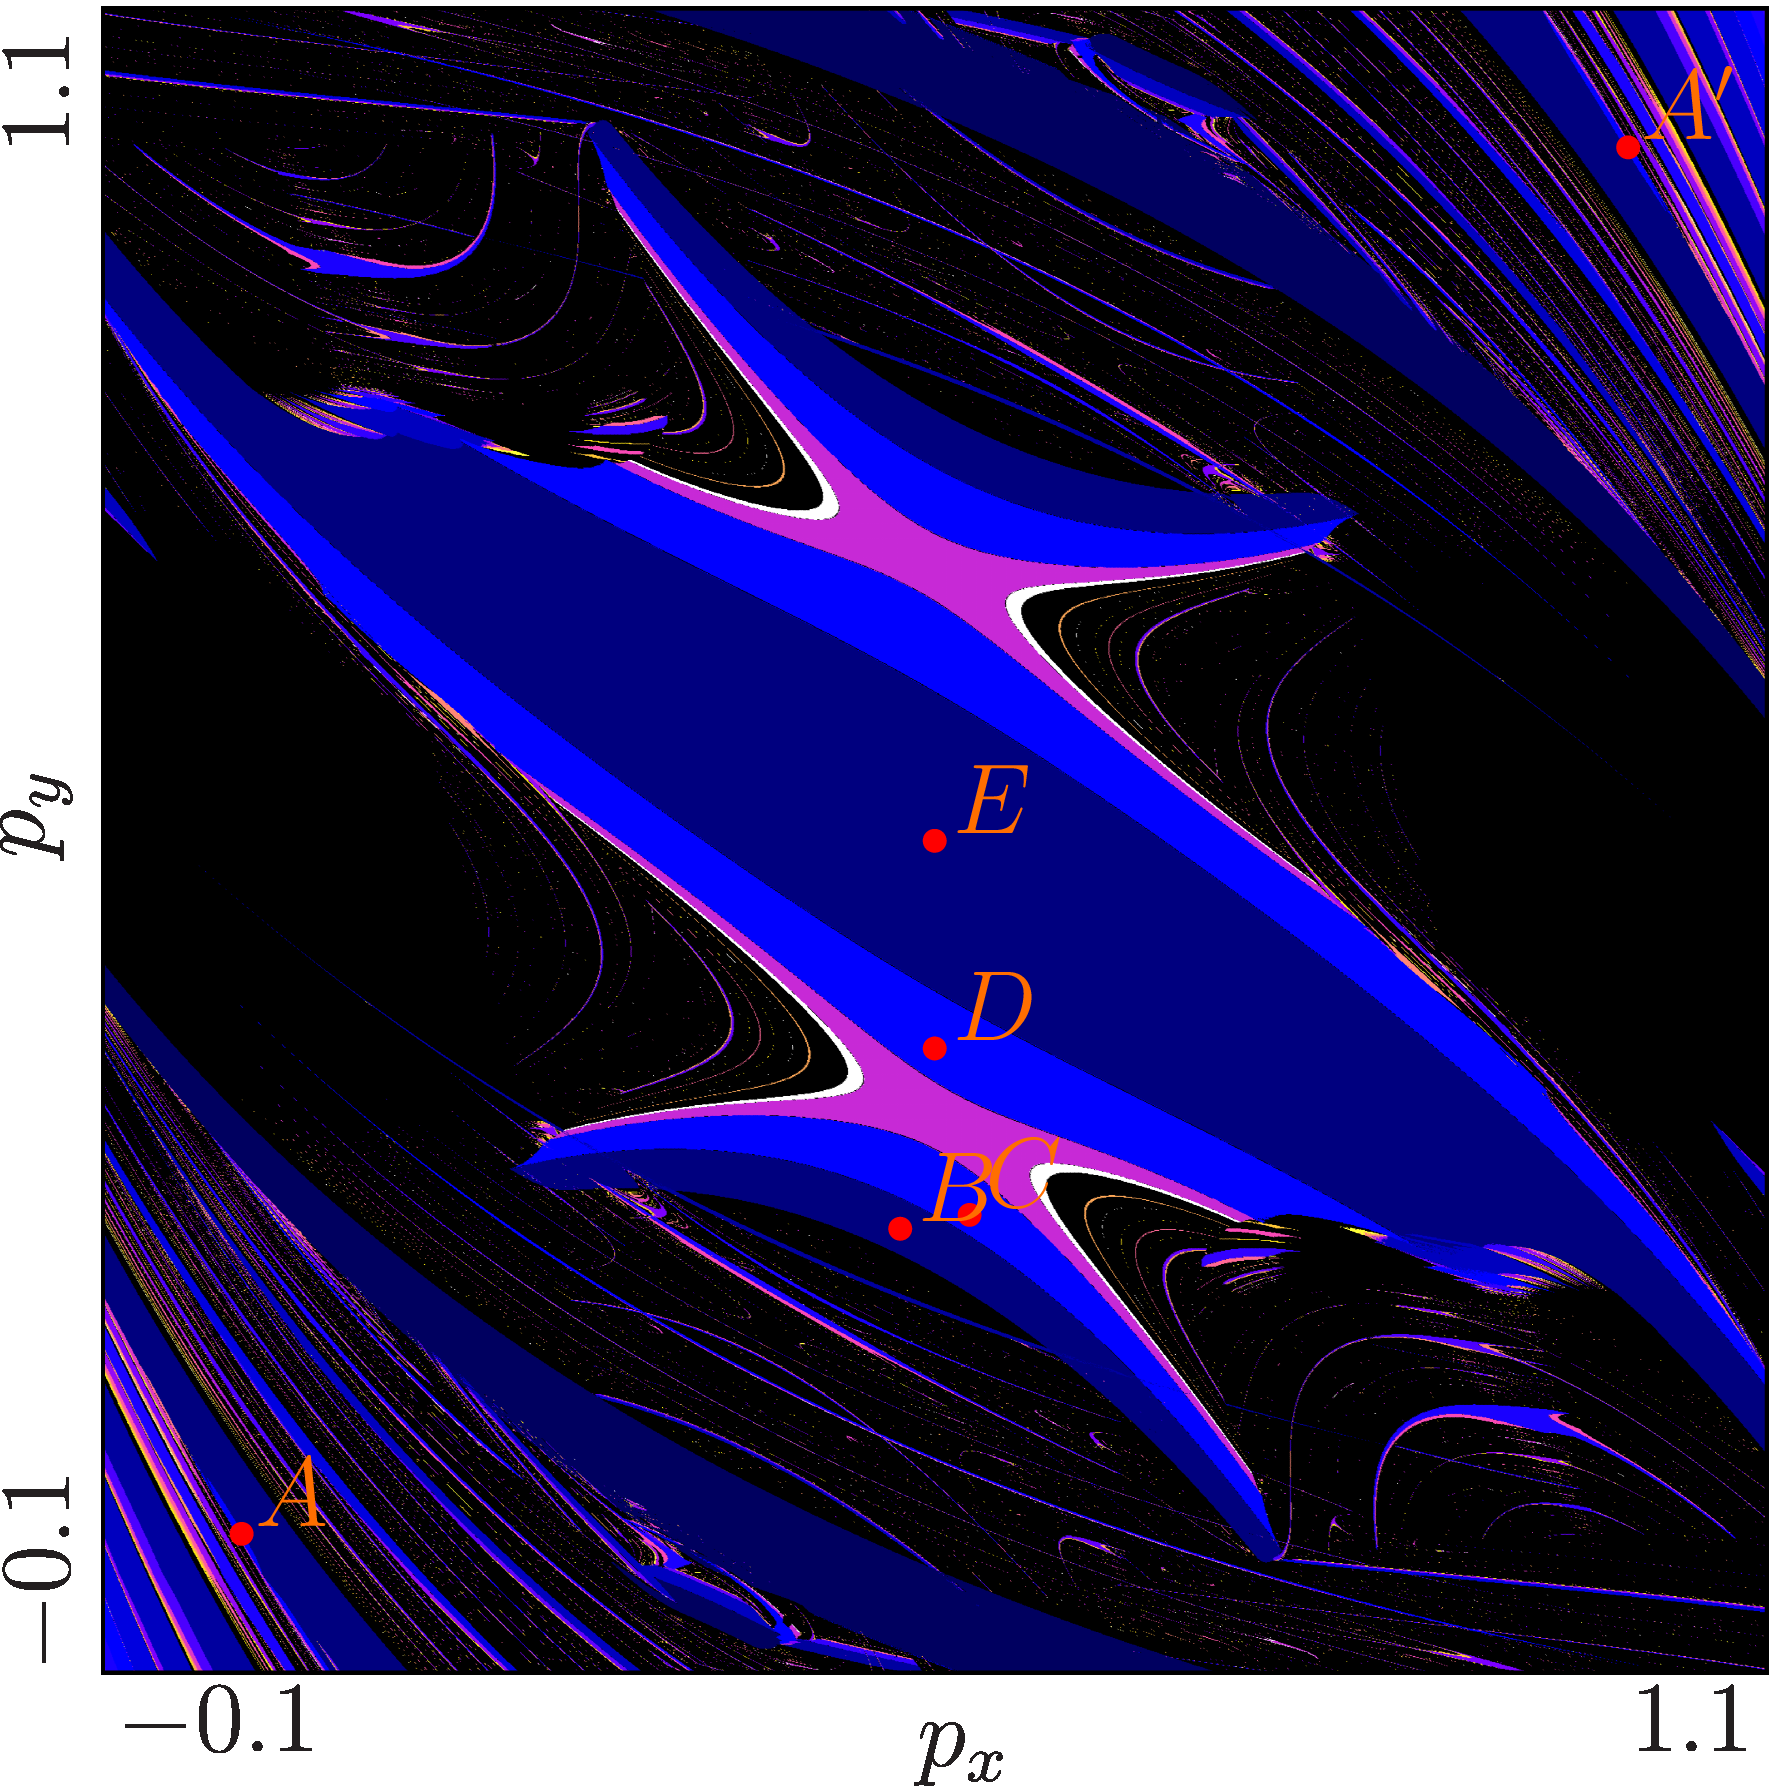
\includegraphics[width=\textwidth]{21_013_Quadratic_2aR1bR_mirror2/2D_Period_Whole/result_halved.png}
        \caption{Halved Model}
        \label{fig:quad.full.2aR1bR_cL_mirr.2.Halved}
    \end{subfigure}
    \caption{2D Period Scans of ...}
    \label{fig:quad.full.2aR1bR_cL_mirr.2.Period}
\end{figure}
